\documentclass{article}

\usepackage{fancyhdr}
\usepackage{extramarks}
\usepackage{amsmath}
\usepackage{amsthm}
\usepackage{amsfonts}
\usepackage{tikz}
\usepackage[plain]{algorithm}
\usepackage{algpseudocode}
\usepackage{enumerate}
\usepackage{tikz}
\usepackage{pythonhighlight}
\usetikzlibrary{automata,positioning}

%
% Basic Document Settings
%  

\topmargin=-0.45in
\evensidemargin=0in
\oddsidemargin=0in
\textwidth=6.5in
\textheight=9.0in
\headsep=0.25in

\linespread{1.1}

\pagestyle{fancy}
\lhead{\hmwkAuthorName}
\chead{\hmwkClass : \hmwkTitle}
\rhead{\firstxmark}
\lfoot{\lastxmark}
\cfoot{\thepage}

\renewcommand\headrulewidth{0.4pt}
\renewcommand\footrulewidth{0.4pt}

\setlength\parindent{0pt}

%
% Create Problem Sections
%

\newcommand{\enterProblemHeader}[1]{
    \nobreak\extramarks{}{Problem \arabic{#1} continued on next page\ldots}\nobreak{}
    \nobreak\extramarks{Problem \arabic{#1} (continued)}{Problem \arabic{#1} continued on next page\ldots}\nobreak{}
}

\newcommand{\exitProblemHeader}[1]{
    \nobreak\extramarks{Problem \arabic{#1} (continued)}{Problem \arabic{#1} continued on next page\ldots}\nobreak{}
    \stepcounter{#1}
    \nobreak\extramarks{Problem \arabic{#1}}{}\nobreak{}
}

\newcommand*\circled[1]{\tikz[baseline=(char.base)]{
		\node[shape=circle,draw,inner sep=2pt] (char) {#1};}}


\setcounter{secnumdepth}{0}
\newcounter{partCounter}
\newcounter{homeworkProblemCounter}
\setcounter{homeworkProblemCounter}{1}
\nobreak\extramarks{Problem \arabic{homeworkProblemCounter}}{}\nobreak{}

%
% Homework Problem Environment
%
% This environment takes an optional argument. When given, it will adjust the
% problem counter. This is useful for when the problems given for your
% assignment aren't sequential. See the last 3 problems of this template for an
% example.
%

\newenvironment{homeworkProblem}[1][-1]{
    \ifnum#1>0
        \setcounter{homeworkProblemCounter}{#1}
    \fi
    \section{Problem \arabic{homeworkProblemCounter}}
    \setcounter{partCounter}{1}
    \enterProblemHeader{homeworkProblemCounter}
}{
    \exitProblemHeader{homeworkProblemCounter}
}

%
% Homework Details
%   - Title
%   - Class
%   - Due date
%   - Name
%   - Student ID

\newcommand{\hmwkTitle}{Homework\ \#10}
\newcommand{\hmwkClass}{Probability \& Statistics for EECS}
\newcommand{\hmwkDueDate}{May 19, 2024}
\newcommand{\hmwkAuthorName}{Fei Pang}
\newcommand{\hmwkAuthorID}{2022533153}


%
% Title Page
%

\title{
    \vspace{2in}
    \textmd{\textbf{\hmwkClass:\\  \hmwkTitle}}\\
    \normalsize\vspace{0.1in}\small{Due\ on\ \hmwkDueDate\ at 23:59}\\
	\vspace{4in}
}

\author{
	Name: \textbf{\hmwkAuthorName} \\
	Student ID: \hmwkAuthorID}
\date{}

\renewcommand{\part}[1]{\textbf{\large Part \Alph{partCounter}}\stepcounter{partCounter}\\}

%
% Various Helper Commands
%

% Useful for algorithms
\newcommand{\alg}[1]{\textsc{\bfseries \footnotesize #1}}
% For derivatives
\newcommand{\deriv}[1]{\frac{\mathrm{d}}{\mathrm{d}x} (#1)}
% For partial derivatives
\newcommand{\pderiv}[2]{\frac{\partial}{\partial #1} (#2)}
% Integral dx
\newcommand{\dx}{\mathrm{d}x}
% Alias for the Solution section header
\newcommand{\solution}{\textbf{\large Solution}}
% Probability commands: Expectation, Variance, Covariance, Bias
\newcommand{\E}{\mathrm{E}}
\newcommand{\Var}{\mathrm{Var}}
\newcommand{\Cov}{\mathrm{Cov}}
\newcommand{\Bias}{\mathrm{Bias}}

\begin{document}

\maketitle

\pagebreak

\begin{homeworkProblem}[1]
    We use python to simulate the result. The code is below:

\begin{python}
    import numpy as np

    # Function to calculate N for a given sample of U values
    def calculate_N(U):
        product = 1
        for i, u in enumerate(U, 1):
            product *= u
            if product < np.exp(-1):
                return i - 1  # Return the index of the last element where the product was less than e^-1
        return len(U)  # If the product never goes below e^-1, return the total count of U values

    # Generate 5000 samples of N
    sample_size = 5000
    Ns = []

    for _ in range(sample_size):
        U = np.random.uniform(0, 1, 1000)  # Generate 1000 uniform random variables
        N = calculate_N(U)
        Ns.append(N)

    # (a) Estimate E(N) using sample mean
    mean_N = np.mean(Ns)
    print("Estimated E(N):", mean_N)

    # (b) Estimate Var(N) using sample variance
    var_N = np.var(Ns)
    print("Estimated Var(N):", var_N)

    # (c) Estimate P(N = i) for i = 0, 1, 2, 3
    counts = np.bincount(Ns)
    probabilities = counts / sample_size
    for i, prob in enumerate(probabilities):
        print("Estimated P(N = {}): {:.4f}".format(i, prob))
\end{python}

Estimated $E(N)$: 0.9896\\
Estimated $Var(N)$: 1.0118918399999999\\
Estimated $P(N = 0)$: 0.3754\\
Estimated $P(N = 1)$: 0.3654\\
Estimated $P(N = 2)$: 0.1780\\
Estimated $P(N = 3)$: 0.0610\\
d. This problem can be related to the sum of exponential random variables through the memoryless property, as $-log(U_i)$ is exponentially distributed with rate 1 (since $U_i \sim Unif(0, 1)$).
Thus the sum up to a certain threshold resemble a Poisson process. And the final distribution of N is a possion distribution with $\lambda = 1$.  
\end{homeworkProblem}


\begin{homeworkProblem}[2]
    We use python to simulate the result. The code is below:
\begin{python}
import numpy as np
import matplotlib.pyplot as plt

def plot_bivariate_normal(rho):
    # Define parameters
    mean = [0, 0]
    cov = [[1, rho], [rho, 1]]  # covariance matrix

    # Generate samples from standard normal distribution
    z = np.random.normal(0, 1, 1000)
    w = np.random.normal(0, 1, 1000)

    # Transform samples to bivariate normal distribution
    x = z
    y = rho * z + np.sqrt(1 - rho**2) * w

    # Plot joint PDF
    plt.figure(figsize=(8, 6))
    plt.hist2d(x, y, bins=30, density=True, cmap='Blues')
    plt.colorbar(label='Probability Density')
    plt.xlabel('X')
    plt.ylabel('Y')
    plt.title('Joint PDF of Bivariate Normal Distribution with ρ = {}'.format(rho))

    # Plot isocontour
    x_range = np.linspace(-3, 3, 100)
    y_range = np.linspace(-3, 3, 100)
    X, Y = np.meshgrid(x_range, y_range)
    Z = np.exp(-(X**2 + Y**2 - 2 * rho * X * Y) / (2 * (1 - rho**2))) / (2 * np.pi * np.sqrt(1 - rho**2))
    plt.contour(X, Y, Z, colors='red', linewidths=1)
    plt.show()

# Generate and plot for each rho value
rhos = [0.1, 0.4, 0.7, 0.9]
for rho in rhos:
    plot_bivariate_normal(rho)

\end{python}

\begin{figure}[htbp]
    \centering
    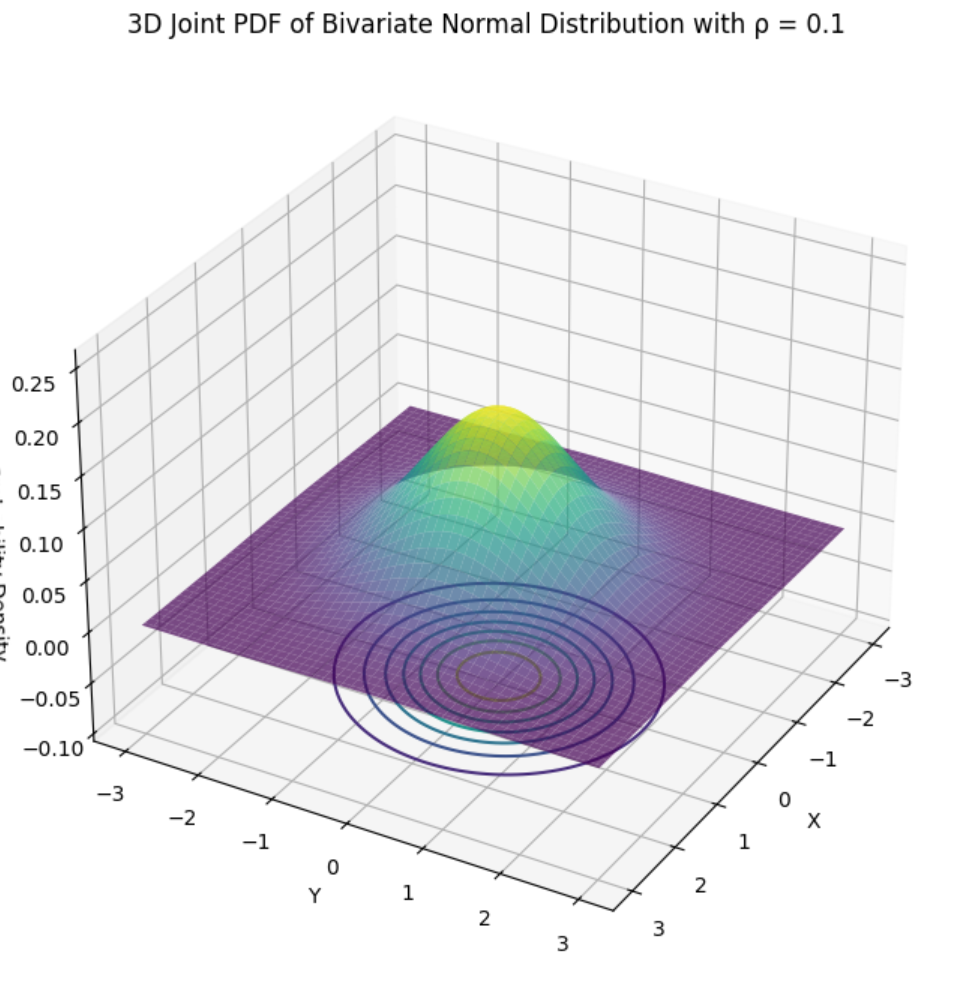
\includegraphics[width=0.23\textwidth]{1.1.png}\hfill
    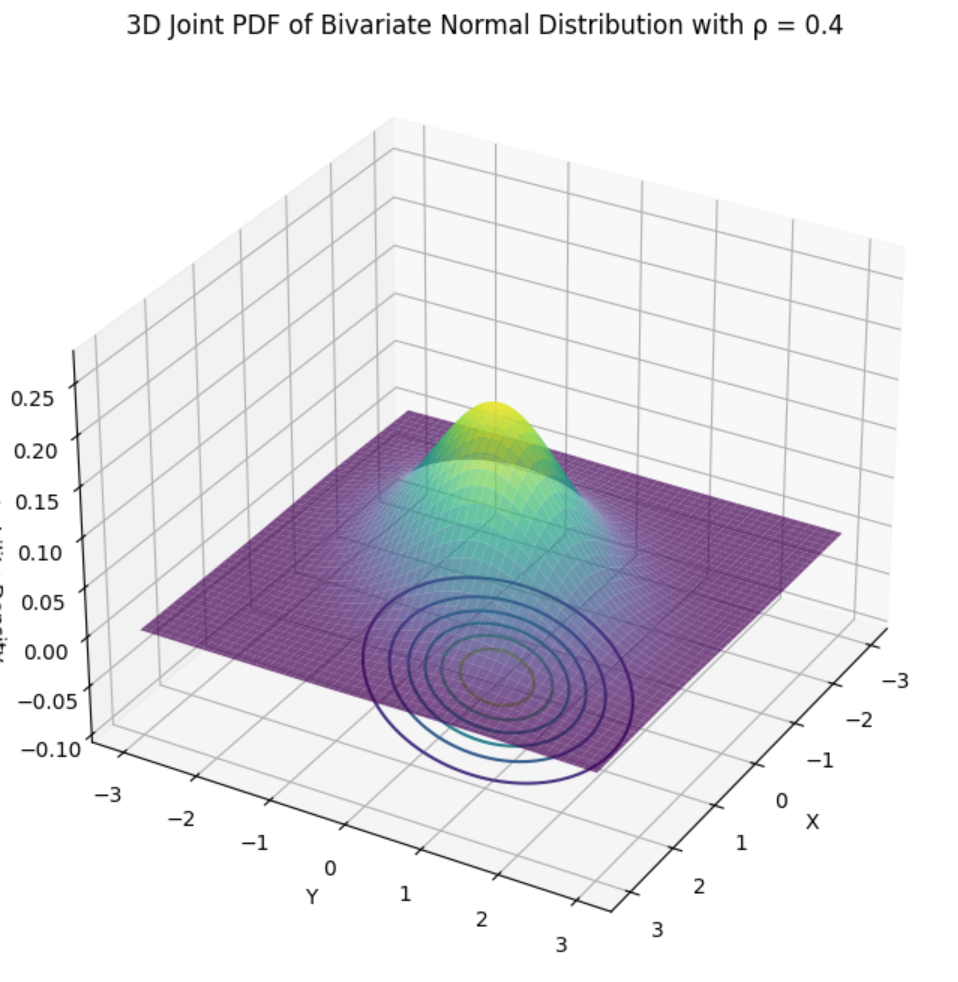
\includegraphics[width=0.23\textwidth]{1.4.png}\hfill
    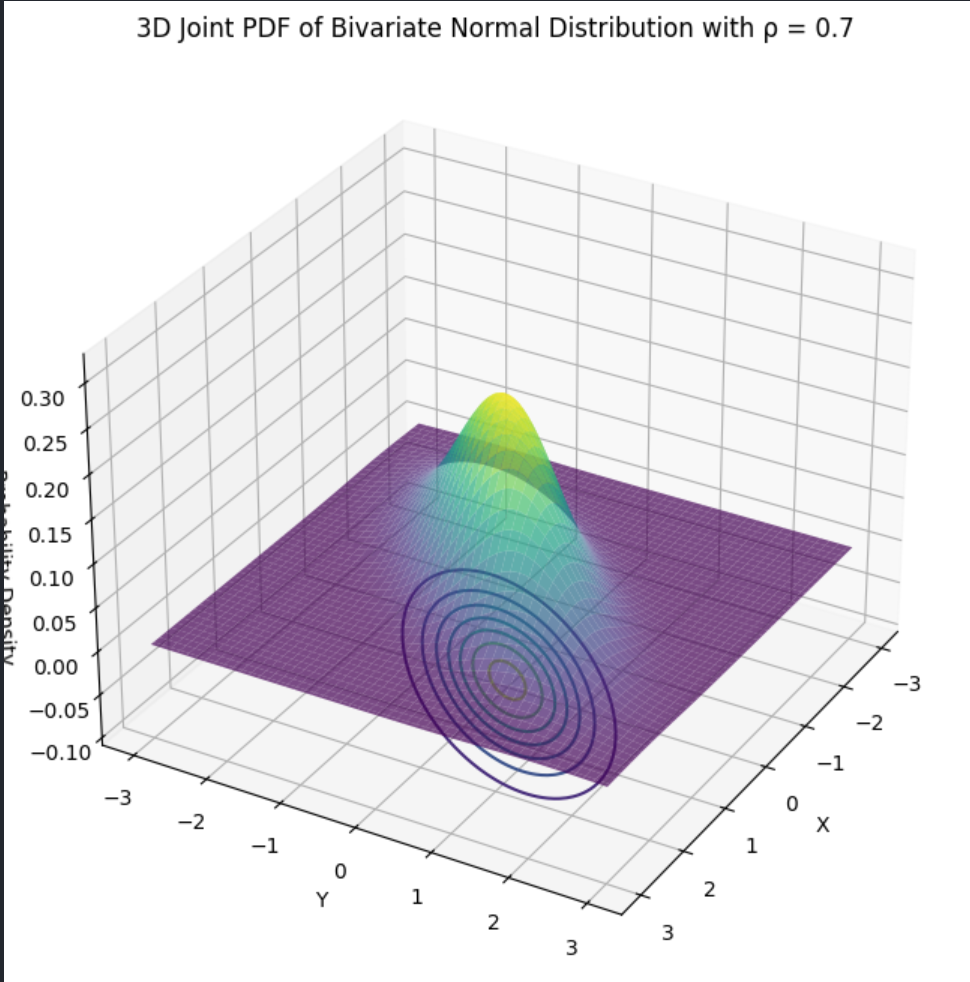
\includegraphics[width=0.23\textwidth]{1.7.png}\hfill
    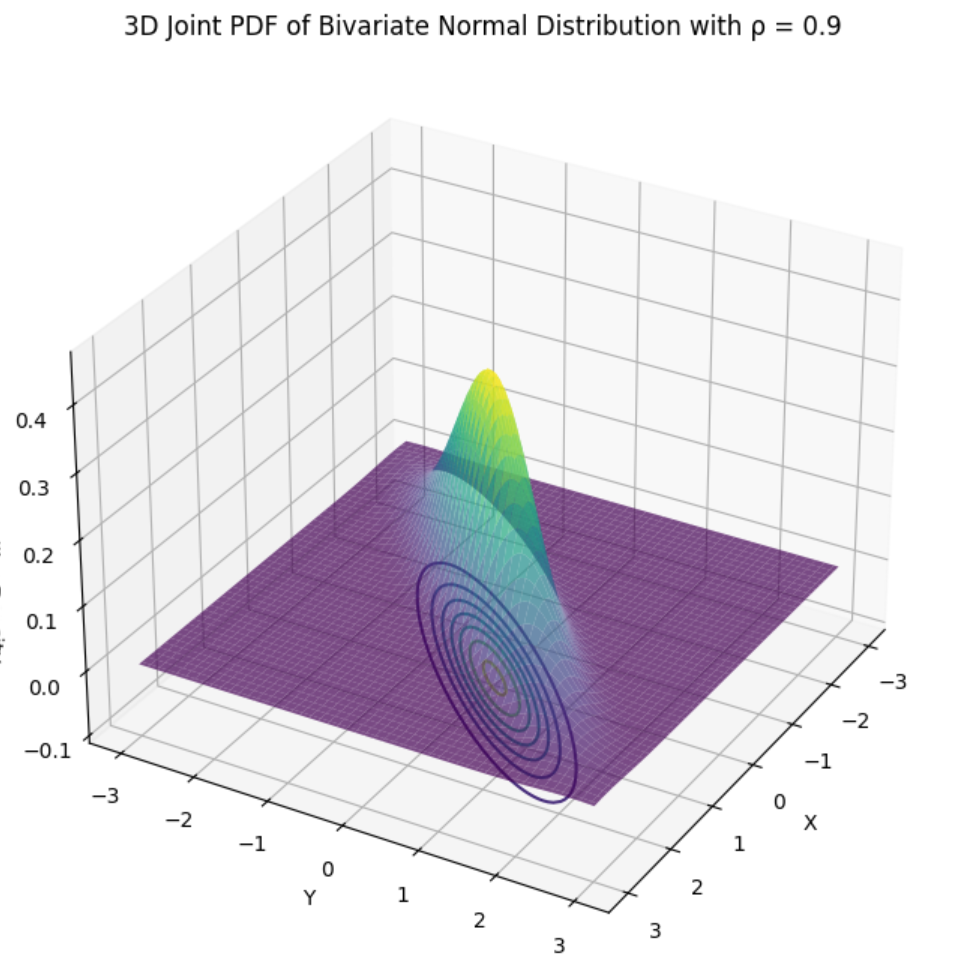
\includegraphics[width=0.23\textwidth]{1.9.png}
    \caption{Bivariate Normal Distributions with Different $\rho$ Values}
    \label{fig:bivariate_normal}
  \end{figure}
 
  

\end{homeworkProblem}



\begin{homeworkProblem}[3]
    \begin{enumerate}[(a)]
    \item 
    According to the memoryless property of exponential distribution, we have $E(X - 2024|X > 2024) = E(X)$. We can obtain the conditional expectation as follows:
    \[
        E(X|X > 2024) = 2024 + E(X - 2024|X > 2024) = 2024 + E(X) = 2023 + \frac{1}{\lambda_1}
    \]

    \item 
    According to the formula of LOTUS:
    \begin{align*}
        &~~~P_1*E(X_1 | X_1 < 1997) + P_2*E(X_1 | X_1 \geq 1997)=E(X_1 )\\
        &(1-e^{-\lambda1997})x + e^{-\lambda1997}(\frac{1}{\lambda} + 1997)= \frac{1}{\lambda}\\
        &x=\frac{1}{\lambda}-\frac{1997e^{-\lambda1997}}{1-e^{-\lambda1997}}
    \end{align*} 
    \item 
    We know that $X_1$, $X_2$, $X_3$ are independent, so we have:\\
    \begin{align*}
        E(X_1 + X_2 + X_3&|X_1 > 1997, X_2 > 2014, X_3 > 2025) = E(X_1|X_1 > 1997, X_2 > 2014, X_3 > 2025)\\
        &+ E(X_2|X_1 > 1997, X_2 > 2014, X_3 > 2025) + E(X_3|X_1 > 1997, X_2 > 2014, X_3 > 2025)\\
        &= E(X_1|X_1 > 1997) + E(X_2|X_2 > 2014) + E(X_3|X_3 > 2025)\\
        &= E(X_1 - 1997|X_1 > 1997) + E(X_2 - 2014|X_2 > 2014) + E(X_3 - 2025|X_3 > 2025) + 6036\\
        &= E(X_1) + E(X_2) + E(X_3) + 6036\\
        &= \frac{1}{\lambda_1} +  \frac{1}{\lambda_2} +  \frac{1}{\lambda_3} + 6036
    \end{align*}

    \end{enumerate}
\end{homeworkProblem}


\begin{homeworkProblem}[4]
\begin{enumerate}[(a)]
    \item 
    \begin{align*}
        f_X(x) &= \int_{-\infty}^{\infty} f_{X, Y}(x, y) \, dy\\
        &= \int_{0}^{\sqrt{x}} 6xy \, dy\\
        &= 3xy^2|_{y=0}^{y=\sqrt{x}}\\
        &= 3x^2
    \end{align*}

    \begin{align*}
        f_Y(y) &= \int_{-\infty}^{\infty} f_{X, Y}(x, y) \, dy\\
        &= \int_{y^2}^{1} 6xy \, dx\\
        &= 3yx^2|_{x=y^2}^{x=1}\\
        &= 3y - 3y^5
    \end{align*}
    Therefore,
    \[
    f_X(x) =
    \begin{cases}
        3x^2, & \text{if } 0 \leq x \leq 1 \\
        0, & \text{otherwise} 
    \end{cases}
    \]
    \[
    f_Y(y) =
    \begin{cases}
        3y - 3y^5, & \text{if } 0 \leq y \leq 1 \\
        0, & \text{otherwise} 
    \end{cases}
    \]
    We can see that $f_{X, Y}(x, y) \neq f_X(x)f_Y(y)$, So $X$ and $Y$ are not independent.

    \item 
    We know that 
    \[
        E[X|Y = y] = \int_{-\infty}^{\infty} xf_{X|Y}(x|y) \,dx    
    \]
    So we first calculate \(f_{X|Y}(x|y)\).
    \[
        f_{X|Y}(x|y) = \frac{f_{X, Y}(x, y)}{f_Y(y)} = \frac{2x}{1 - y^4}, \ y^2 \leq x \leq 1.  
    \]
    \[
        E[X|Y = y] = \int_{-\infty}^{\infty} xf_{X|Y}(x|y) \,dx = \int_{y^2}^{1} x\frac{2x}{1 - y^4} \,dx = \frac{2}{3} \cdot \frac{1 + y^2 + y^4}{1 + y^2}   
    \]
    Next, we calculate $E[X^2|Y = y]$.
    \[
        E[X^2|Y = y] = \int_{-\infty}^{\infty} x^2f_{X|Y}(x|y) \,dx = \int_{y^2}^{1} x^2\frac{2x}{1 - y^4} \,dx = \frac{1 + y^4}{2}  
    \]
    So we have:
    \[
        Var[X|Y = y] =  E[X^2|Y = y] -  (E[X|Y = y])^2 = \frac{1 + y^4}{2} - \frac{4}{9} \cdot \frac{(1 + y^2 + y^4)^2}{(1 + y^2)^2} 
    \]

    \item
    According to $b$, we have:
    \[
        E[X|Y] = \frac{2}{3} \cdot \frac{1 + Y^2 + Y^4}{1 + Y^2}  
    \]
    \[
        Var[X|Y] = \frac{1 + Y^4}{2} -\frac{4}{9} \cdot \frac{(1 + Y^2 + Y^4)^2}{(1 + Y^2)^2}  
    \]
\end{enumerate}
\end{homeworkProblem}


\begin{homeworkProblem}[5]

\begin{enumerate}[(a)]
    \item 
    The PMF of $X$ is $P(X = k) = p(1 - p)^k$. So we have:
    \begin{align*}
        H(X) &= -\sum_{k = 0}^{\infty} p(1 - p)^k log(p(1 - p)^k)\\
        &= -log_2 p - \frac{1 - p}{p} log_2 (1 - p)
    \end{align*}  

    \item 
    Through LOTP, we have:
    \[
        P(X = Y) = \sum_{k = 0}^{\infty} P(X = k) \cdot P(Y = k) = \sum_{k = 0}^{\infty} p_k^2    
    \]
    Define $Z$ so that $P(Z = p_k) = p_k$, so we have:
    \[
        E(Z) = \sum_{k = 0}^{\infty} p_k \cdot p_k = P(X = Y)    
    \]
    According to Jensen's inequality:
    \[
        E(log(Z)) \leq log(E(Z))    
    \]
    \[
        \sum p_k log_2 p_k \leq log_2 \sum p_k^2    
    \]
    \[
        -H(X) \leq log_2 P(X = Y)    
    \]
    \[
        P(X = Y) \geq 2^{-H(X)}    
    \]
\end{enumerate}

\end{homeworkProblem}


\begin{homeworkProblem}[6]
    $X_i \sim Bern(p)$, so we have $E(X_i) = p$, $Var(X_i) = p(1 - p)$, $E[\hat{p}] = p$, $Var[\hat{p}] = \frac{p(1 - p)}{N}$.

    Also, we have $P(|\hat{p} - p| \geq \epsilon) \leq \delta$.
\begin{enumerate}[(a)]
    \item 
    Applying Chebyshev's inequality on random variable $\hat{p}$, we have
    \[
        P(|\hat{p} - p| \geq \epsilon) \leq \frac{p(1 - p)}{N\epsilon ^2} \rightarrow \delta = \frac{p(1 - p)}{N\epsilon ^2}, \ \epsilon = \sqrt{\frac{p(1 - p)}{N\epsilon}}
    \] 
    Therefore, we know that $\delta$ negatively correlates with$\epsilon$, i.e., given a fixed number of samples N, there is
    natural trade-off between accuracy and confidence. Besides, 1. Fix the confidence interval parametrized
    by $\delta$, reducing the estimation error $\epsilon$ requires increasing the number of samples N. 2. Fix the estimation
    error $\epsilon$, narrowing the confidence interval requires increasing the number of samples N. The
    impacts of N is on both the “estimation accuracy” and “estimation confidence”.
    \item 
    Applying Hoeffding's inequality on random variable $\hat{p}$, we have
    \[
        P(|\hat{p} - p| \geq \epsilon) \leq 2e^{-2N\epsilon^2} \rightarrow \delta = 2e^{-2N\epsilon^2}, \ \epsilon = \sqrt{\frac{ln(2/\delta)}{2N}}
    \] 
    The explanation is the same in $(a)$.

    \item 
    Chebyshev's inequality:\\
    • Pros: 1. sharp bound and cannot be improved in general.\\
    2. can be improved with extra distributional information on polynomial moments.\\
    • Cons: 1. requires the existence of moments until the second order. \\
    2. quadratic convergence rate.\\
    Hoeffding's inequality:\\
    • Pros: 1. exponential convergence rate. 2. does not require assumption on moments.
    • Cons: 1. works only for sub-Gaussian. 2. in general not sharp when the variance is small.
\end{enumerate}
\end{homeworkProblem}


\end{document}
